\section{Elektrotechnik}
\subsection{Electric Circuit III}

\subsubsection{Passive Sign Convention}
The convention defines electric power flowing out of the circuit into an electrical component as positive, and power flowing into the circuit out of a component as negative.

\subsubsection{Nodal analysis}

\subsubsection{Mesh analysis}

\subsubsection{Thévenin's theorem}

Any linear electrical network with voltage and current sources and only resistances can be replaced at terminals A-B by an equivalent voltage source $V_{th}$ in series connection with an equivalent resistance $R_{th}$.

\subsubsection{Norton's theorem}

Any linear electrical network with voltage and current sources and only resistances can be replaced at terminals A-B by an equivalent current source $I_{NO}$ in parallel connection with an equivalent resistance $R_{NO}$.

\subsubsection{Line Voltage/Phase Voltage}

Line voltage is the voltage measured between any two lines in a three-phase circuit. Phase voltage is the voltage measured across a single component in a three-phase source or load.

For ``Y'' circuits:
\begin{align*}
  E_{line}&=\sqrt{3}E_{phase} \\
  I_{line}&=I_{phase}
\end{align*}

For $\Delta$ circuits:

\begin{align*}
  E_{line}&=E_{phase} \\
  I_{line}&=\sqrt{3}I_{phase}
\end{align*}

\subsection{Introduction to Analog Electronic Technology I}

In this course we learned semiconductor diodes and Bipolar Junction Transistor, and basic amplifying circuits. We also learned the operational amplifying circuits and the feedback.

\paragraph{PN Junction} PN junctions are elementary "building blocks" of most semiconductor electronic devices such as diodes, transistors. A PN junction is a boundary or interface between p-type and N-type.

After joining p-type and n-type semiconductors, electrons from the n region near the PN interface tend to diffuse into the p region. As electrons diffuse, they leave positively charged ions (donors) in the n region. Likewise, holes from the p-type region near the p–n interface begin to diffuse into the n-type region, leaving fixed ions (acceptors) with negative charge. The regions nearby the p–n interfaces lose their neutrality and become charged, forming the space charge region or depletion layer. Its resistance is very big.

\paragraph{Transistor} A bipolar junction transistor (BJT or bipolar transistor) is a type of transistor that relies on the contact of two types of semiconductor for its operation.
BJTs come in two types, or polarities, known as PNP and NPN. The regions of a BJT are called emitter, collector, and base.

\paragraph{Filter} Passive filters are based on combinations of resistors (R), inductors (L) and capacitors (C). Because they do not depend on an external power supply and/or they do not contain active components such as transistors.

\subsection{Analog Electronics Experiments}

\newpage 
\subsection{Fundamental Technology of Digital Electronics I}

\newpage

\subsection{Curriculum Design of Electronics II}

The student grouped to design a digital frequency meter. The structure is shown in figure \ref{fig_digit_meter}.

\begin{figure}
  \centering
  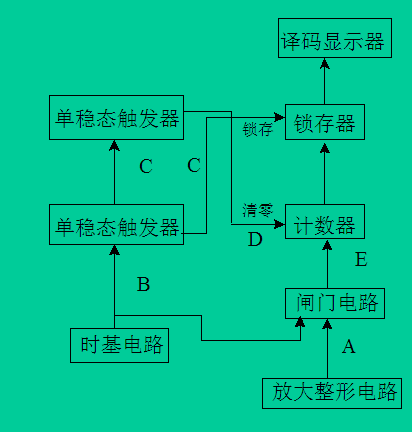
\includegraphics[width=2.3in]{fig/curriculum_circuit_design.png}
  \caption{Digital Frequency Meter}\label{fig_digit_meter}
\end{figure}

\subsection{High Frequency Electronic Circuit}
High Frequency ranges from \SIrange{0.3}{300}{\mega\hertz}. I learnt from this course the general structure of a radio communication system, it is composed of transmitter and receiver. The course mainly focus on the following:
\begin{enumerate}
  \item Signal Amplifying

  small-signal RF amplifier, RF power amplifier

  \item Signal Generation

  oscillator

  \item Signal Modulation

  frequency modulation, phase modulation

  \item Feedback Control

  phase lock loop
\end{enumerate}
\subsubsection{Signal Amplifying}

\paragraph{Resonant Circuit} Resonant circuit eliminate the unwanted frequencies due to the nonlinearty of components. The loaded Q-factor is a measure of the selectivity of a resonant circuit:

$$Q=\frac{f_{center}}{\Delta f}=\frac{R_p}{X_p}$$

\begin{figure}
  \centering
  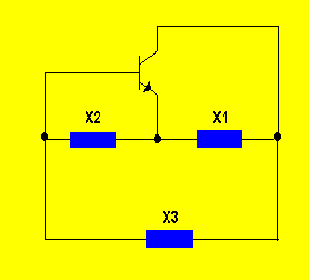
\includegraphics[width=1.5in]{fig/fig_LC_resonant.png}
  \caption{LC Resonant Circuit, $|X_3|=|X_1+X_2|$ and $X_1+X_2+X_3=0$.}\label{fig_lc_resonant}
\end{figure}

\paragraph{Small-Signal RF Amplifier} We can module a small-signal RF transistor as a two-port network with Y-parameters, as shown in firugre \ref{fig_rf_signal_amp}. The input port of transistor is transformer's secondary winding.

\begin{figure}
  \centering
  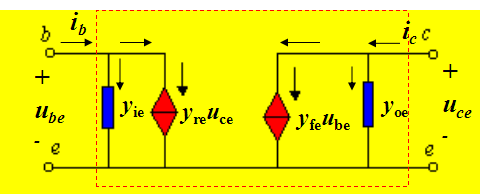
\includegraphics[width=2.5in]{fig/fig_rf_signal_amp.png}
  \caption{Small-Signal RF Amplifier Equivalent Circuit}\label{fig_rf_signal_amp}
\end{figure}

\paragraph{RF Power Amplifier} The RF power amplifier takes a low power input and regenerates the signal at several watts higher. Various types of power amplifiers are classified by the amount of time that the transistors conduct.

\subparagraph{Conduction Angle} Conduction angle($\phi_c$) is related to efficiency in RF power amplifier design, and the amplifier are classified according to its conduction angle.

\begin{itemize}
  \item Class-A: \SI{360}{\degree}, broad band
  \item Class-AB: approximately larger than \SI{180}{\degree}, broad band
  \item Class-C: smaller than \SI{180}{\degree} with efficiencies up to 90\%, narrow band
\end{itemize}

\begin{figure}
  \centering
  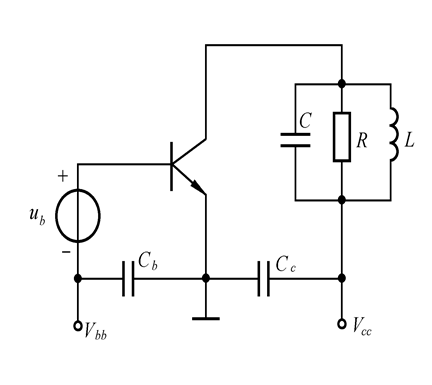
\includegraphics[width=1.8in]{fig/fig_rf_power_amp.png}
  \caption{RF Power Amplifier Load is resonant circuit}\label{fig_rf_power_amp}
\end{figure}

\subsubsection{Signal Generation}

\paragraph{LC oscillator} An Oscillator is basically an Amplifier  with ``Positive Feedback'', LC Oscillators are commonly used in radio-frequency circuits because of their good \emph{phase noise characteristics} and their \emph{ease of implementation}.

$$f=\frac{1}{2\pi \sqrt{LC}}$$

\begin{figure}
  \centering
  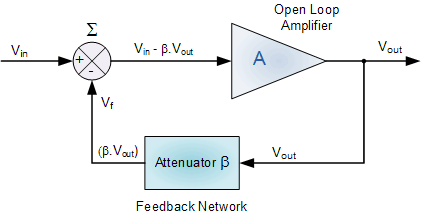
\includegraphics[width=2.0in]{fig/osc35.png}
  \caption{Block diagram of a feedback linear oscillator}\label{osc_diag}
\end{figure}

\subsubsection{Signal Modulation}

\paragraph{AM} The amplitude of the \emph{carrier wave} is varied in proportion to the waveform being transmitted. Set $c(t)=A\cdot sin(2\pi f_c t)$ as a carrier wave, and $m(t) = M \cdot cos(2 \pi f_m t + \Phi)$ is the modulation waveform. The amplitude modulated signal is:

\begin{align*}
  y(t) &= [ 1+ m(t)] \cdot c(t) \\
       &= A \cdot [ 1 + M ] \cdot cos(2 \pi f_m t + \Phi ) \cdot sin(2 \pi f_c t )
\end{align*}

\subparagraph{Envelope Detector} An envelope detector can be used to demodulate a previously modulated signal by removing all high frequency components of the signal, the corresponding circuit is shown in figure \ref{fig_rectified_voltagemeter}.

\paragraph{FM} Frequency Modulation (FM) is the encoding of information in a carrier wave by varying the instantaneous frequency of the wave. The frequency modulated signal is
$$u_{FM}(t)=Ucos[\omega_c t + k_f \int_{0}^{t} u_\Omega (t) dt]$$

\subparagraph{Direct Modulation} Direct FM modulation can be achieved by directly feeding the message into the input of a VCO.

\subparagraph{Ratio Detector} The ratio detector is not affected by amplitude variations on the FM wave. The output of the detector adjusts itself automatically to the average amplitude of the input signal.

The process of a ratio detector is:

$$FM\xrightarrow[\text{phase shift network}]{\text{frequency sensitive}}FM-PM\xrightarrow[]{\text{FM-PM + FM}}FM-AM\xrightarrow[\text{detector}]{\text{envelope}}u_\Omega(t)$$

\begin{figure}
  \centering
  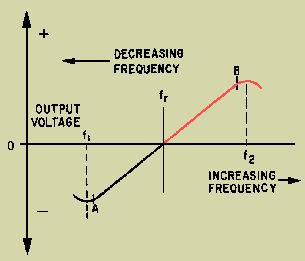
\includegraphics[width=2.5in]{fig/0260.png}
  \caption{Discriminator response curve}\label{fig_discriminator_respc}
\end{figure}

It uses a double-tuned RF transformer to convert frequency variations in the received FM signal to amplitude variations(\textbf{AM-FM}). A typical discriminator response curve is shown in figure \ref{fig_discriminator_respc}.

\subparagraph{Modulation Index} The value of the modulation index indicates by how much the modulated variable varies around its unmodulated level. It relates to variations in the carrier frequency:

$$h = \frac{\Delta{}f}{f_m} = \frac{f_\Delta |x_m(t)|}{f_m} $$

where $f_m$ is the highest frequency component present in the modulating signal $x_m(t)$ and $\Delta{}f$ is the peak frequency-deviation.

\paragraph{Mixer} RF mixing enables signals to be converted to different frequencies and thereby allowing the signals to be processed more effectively.

\begin{figure}
  \centering
  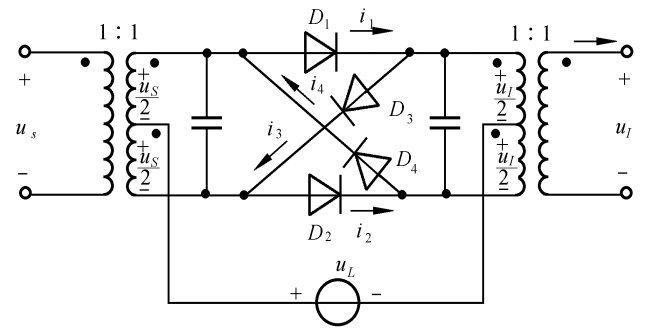
\includegraphics[width=3.2in]{fig/double-balanced-mixer.png}
  \caption{Basic double balanced diode mixer circuit}\label{fig_mixer}
\end{figure}

\begin{align*}
  i'  &= i_1-i_2=g_dk(\omega_Lt)(u_S-u_I) \\
  i'' &= i_3-i_4=g_dk(\omega_Lt-\pi)(u_S+u_I) \\
  i_I &= g_dU_{sm}\cos\omega_st-\frac{2}{\pi}g_dU_{Im}\cos\omega_st
\end{align*}

\subsubsection{Feedback Control}
\paragraph{PLL} A phase-locked loop (PLL) is a control system that generates an output signal whose phase is related to the phase of an input signal.
\begin{figure}
  \centering
  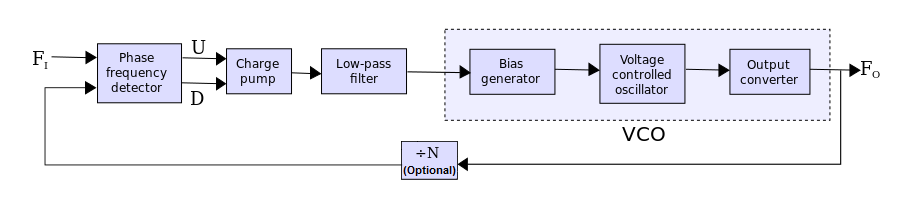
\includegraphics[width=4.5in]{fig/PLL_generic_inline_optional_N.png}
  \caption{Block diagram of a phase-locked loop}\label{fig_PLL}
\end{figure}

\paragraph{DDS} Direct Digital Synthesizer (DDS) is a type of frequency synthesizer used for creating arbitrary waveforms from a single, fixed-frequency reference clock.

\begin{figure}
  \centering
  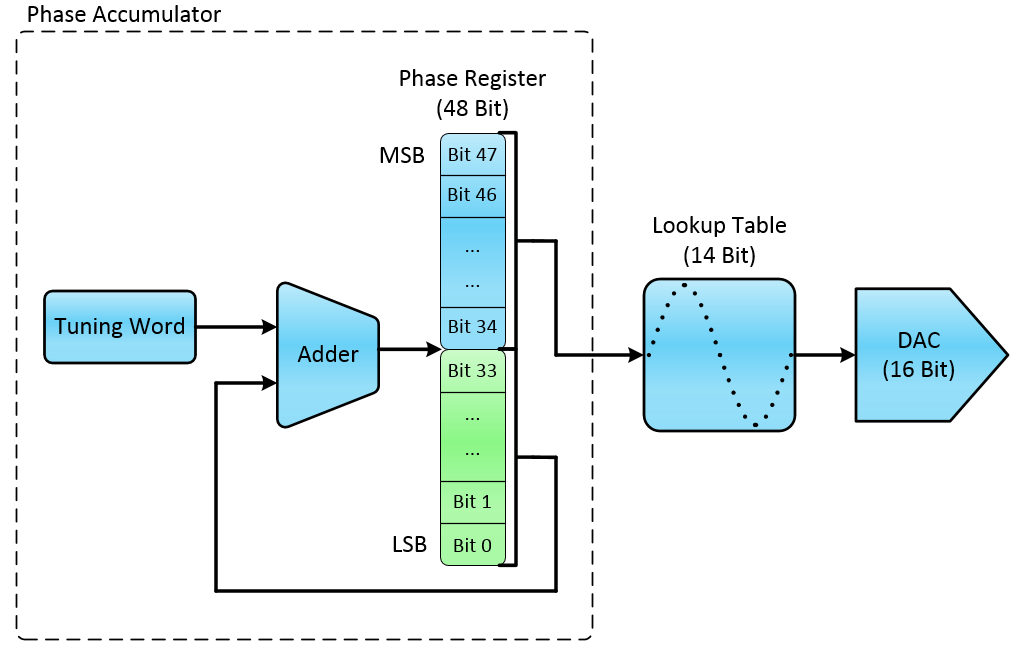
\includegraphics[width=3.5in]{fig/Fig_2_DDS_Block_Diagram.png}
  \caption{Hardware Block Diagram for the DDS Architecture}\label{fig_DDS}
\end{figure}

\subparagraph{Lookup Table}

The output of the phase register only looks like a digital ramp as the memory address increases over time, which is changing at the rate specified by the \emph{tuning word}. 